\documentclass[a4paper,12pt]{extarticle}
\usepackage[utf8]{inputenc}
\usepackage[francais]{babel}
\usepackage[T1]{fontenc}
\usepackage[pdftex]{graphicx}
\usepackage{url}
\usepackage{caption}
\usepackage{graphicx}
\usepackage{multirow}

\usepackage{fancyhdr}
\pagestyle{fancy}






\setlength{\parindent}{0cm}
\setlength{\parskip}{1ex plus 0.5ex minus 0.2ex}
\newcommand{\hsp}{\hspace{20pt}}
\newcommand{\HRule}{\rule{\linewidth}{0.5mm}}
%opening

\renewcommand{\headrulewidth}{1pt}
\fancyhead[L]{\leftmark}
\fancyhead[R]{}

\renewcommand{\footrulewidth}{1pt}
\fancyfoot[C]{\textbf{page \thepage}} 




\begin{document}

\begin{titlepage}
  \begin{sffamily}
  \begin{center}

    % Upper part of the page. The '~' is needed because \\
    % only works if a paragraph has started.
    %\includegraphics[scale=1]{univangers.jpg}~\\[1.5cm]

    \textsc{\LARGE Université d'Angers}\\[2cm]

   

    % Title
    \HRule \\[0.4cm]
    { \huge \bfseries Stage en entreprise}{\bfseries  \\[0.4cm] }

    \HRule \\[2cm]
    
    % Image
	\begin{center}
		
\includegraphics[scale=1]{Img/logo/logo_fleurymichon}
	\end{center}
    
    % Author and supervisor
    \begin{minipage}{0.4\textwidth}
      \begin{flushleft} \large
        FRESNEAU \textsc{Quentin}
      \end{flushleft}
    \end{minipage}
    

    \vfill
    \HRule\\[2cm]
    % Bottom of the page
    {\large 26 Avril 2017}

  \end{center}
  \end{sffamily}
\end{titlepage}
\clearpage

\tableofcontents

\clearpage

\section{Remerciements}

\paragraph{}
à voir\\

\clearpage

\section{Introduction}

\paragraph{}
à voir\\

\clearpage

\section{Présentation de l’entreprise}

\subsection{Historique du groupe}

\paragraph{}
à voir\\

\subsection{L’entreprise Fleury Michon}

\paragraph{}
à voir\\

\subsection{Situation géographique}

\paragraph{}
à voir\\

\centerline{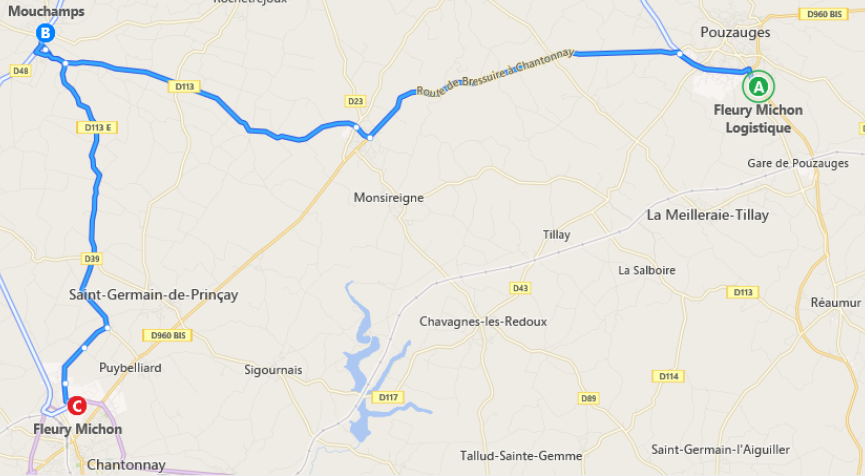
\includegraphics[scale=0.40]{Img/Img_SituationGeo}}

\subsection{Présentation de l'équipe et des locaux}

\paragraph{}
à voir\\

\clearpage

\section{Présentation du projet de stage}

\subsection{Analyse du besoin}

\paragraph{}
à voir\\

\subsection{But du projet}

\paragraph{}
à voir\\

\clearpage

\section{Élaboration du projet}

\subsection{Partage du travail}

\paragraph{}
à voir\\

\subsection{Matériel mis à disposition}

\paragraph{}
à voir\\

\subsection{Réalisation hors rapport}

\paragraph{}
GIT du projet :
\url{https://github.com/qfresneau/Stage}\\

\clearpage

\section{Développement}

\paragraph{}
à voir\\

\clearpage

\section{État final du projet}

\paragraph{}
à voir\\

\clearpage

\section{Conclusion}

\paragraph{}
à voir\\

\clearpage

\section{Sources}

\paragraph{}
à voir\\

\section{Glossaire}

\paragraph{}
à voir\\

\clearpage

\section{Annexes}

\begin{center}
%\includegraphics[scale=0.6, angle=270]{Gantt4}
\end{center}

\end{document}
\newline


